\chapter{Intermolekulare Kräfte}
\section{Van-Der-Waals-Kräfte}

\begin{itemize}
	\item<+-> Schwache Wechselwirkungen zwischen verschiedenen Atomen oder Molekülen
	\item<+-> Entstehung durch kurzzeitige Dipolmomente aufgrund ungleichmäßiger Elektronenverteilung um den Atomkern
	\item<+-> Unterteilt in drei Unterarten
\end{itemize}
\begin{block}<+->{Stärke}
	Van-der-Waals-Kräfte sind generell sehr schwache Kräfte
\end{block}


\subsection{London-Kräfte}

\begin{itemize}
	\item<+-> Spontane Polarisation von Teilchen ($e^-$ \say{schwirren} gerade auf einer Seite)
	\item<+-> Induzierte Dipole in benachbarteten Teilchen
	\item<+-> Zwischen nicht-dipolen
	\item<+-> $\implies$ Teilchen ziehen sich an / stoßen sich ab
\end{itemize}
\begin{block}<+->{Stärke}
	Sehr schwach
\end{block}


\subsection{Debye-Wechselwirkung}

\begin{itemize}
	\item<+-> Bereits existierende Dipole in der Lösung
	\item<+-> Induzierte Dipole in benachbarteten Teilchen
	\item<+-> Zwischen Dipol und nicht-dipol
	\item<+-> $\implies$ Teilchen ziehen sich an / stoßen sich ab
\end{itemize}
\begin{block}<+->{Stärke}
	Sehr schwach, aber generell stärker als London-Kräfte
\end{block}



\subsection{Keesom-Kraft}

\begin{itemize}
	\item<+-> Bereits existierende Dipole in der Lösung
	\item<+-> Besagte Dipole ziehen sich an / stoßen sich ab.
	\item<+-> Zwischen zwei Dipolen
\end{itemize}
\begin{block}<+->{Stärke}
	Sehr schwach, aber generell die stärkste der drei Van-der-Waals-Kräfte
\end{block}


\section{Wasserstoffbrückenbindungen}

\chemfig{R^1-\charge{45:6pt=$\delta^-$}{X}-\charge{45:6pt=$\delta^+$}{H}-[:0,,,,dotted]\charge{180=\|,45:6pt=$\delta^-$}{Y}-R^2}
\begin{itemize}
	\item<+-> Zwischen Wasserstoffatom und stark elektronegativem Atom (\chemfig{O}, \chemfig{N}, \chemfig{F}, ...)
	\item<+-> Insbesondere an freiem Valenzelektronenpaar
\end{itemize}
\begin{block}<+->{Stärke}
	Schwächer als Ionenbindung, Kovalente Bindung, etc. aber deutlich stärker als Van-der-Waals-Kräfte
\end{block}
\begin{examples}<+->
\chemfig{HO-H-[:0,,,,dotted]\charge{180=\|,90=\|}{O}H_2}
\end{examples}


\chapter{Reaktionsmechanismen}
\section{Grundlagen}
\subsection{induktive Effekte}

\begin{itemize}
	\item<+-> Elektronenverschiebungen entlang konvalenter Bindungen
	\item<+-> Bindungen mit Elektronegativtätsdifferenzen (aber keine Ionenbindung) (z.B. \ch{C-F})
	\item<+-> Beeinflusst Abspaltbarkeit von Teilmolekülen in z.B. nukleophiler Substitution ($S_N1$), elektrophiler Addition, ... (schwächt Bindung)
\end{itemize}
\pause
Zum Beispiel durch folgende Gruppen
\begin{columns}
\begin{column}{0.48\textwidth}
\begin{block}{$+\text{I}$-Effekt (Schiebend)}
\begin{itemize}
	\item t-Butylgruppe (\ch{-C(CH_3)_3})
	\item i-Propylgruppe (\ch{-CH(CH_3)_2})
	\item Alkylrest (\ch{-R})
\end{itemize}
\end{block}
\begin{examples}<+->
\chemfig{H_3\charge{[overlay=false]90:5pt=$\delta^-$}{C}-\charge{[overlay=false]90:5pt=$\delta^+$}{Li}}
\end{examples}
\end{column}
\begin{column}{0.48\textwidth}
\begin{block}{$-\text{I}$-Effekt (Ziehend)}
\begin{itemize}
	\item Hydroxygruppe (\ch{-OH}) / Carbonylgruppenteil (\ch{-C=O})
	\item Iodatom (\ch{-I}) / Bromatom (\ch{-Br}) / Chloratom (\ch{-Cl}) / Fluoratom (\ch{-F})
	\item Nitrogruppe (\ch{-NO_2}) / Aminogruppe (\ch{-NH_2}) / Carboxygruppe (\ch{-NH_2}) / Cyanogruppe (\ch{-CN}) / Sulfonylgruppe (\ch{-SO_3H})
\end{itemize}
\end{block}
\begin{examples}<+->
\chemfig{H_3\charge{[overlay=false]90:5pt=$\delta^+$}{C}-\charge{[overlay=false]90:5pt=$\delta^-$}{Br}}
\end{examples}
\end{column}
\end{columns}


\subsection{Reaktionsenthalpie}

	\begin{block}{Was ist das?}
	\begin{itemize}
		\item<+-> $\Delta H_R$ gibt die Änderung der Enthalpie ($\approx$Energie) im Verlauf einer Reaktion an, bei konstantem Druck
		\item<+-> Sie entspricht der Differenz zwischen Produkt und Edukt: $\Delta H_R = H_{\text{Produkt}} - H_{\text{Edukt}}$
		\item<+-> Da sie nur vergleichbar ist, wenn die Bedingungen gleich sind, verwendet man Standardbedingungen ($273,15 K$, $1 \text{Bar}$)
		\item<+-> Die Reaktionsenthalpie unter Standardbedingungen wird als $\Delta H_R^0$ bezeichnet.
	\end{itemize}
	\end{block}


	\begin{columns}
	\begin{column}{0.48\textwidth}
	\begin{block}{Exotherm}
	\begin{figure}[H]
		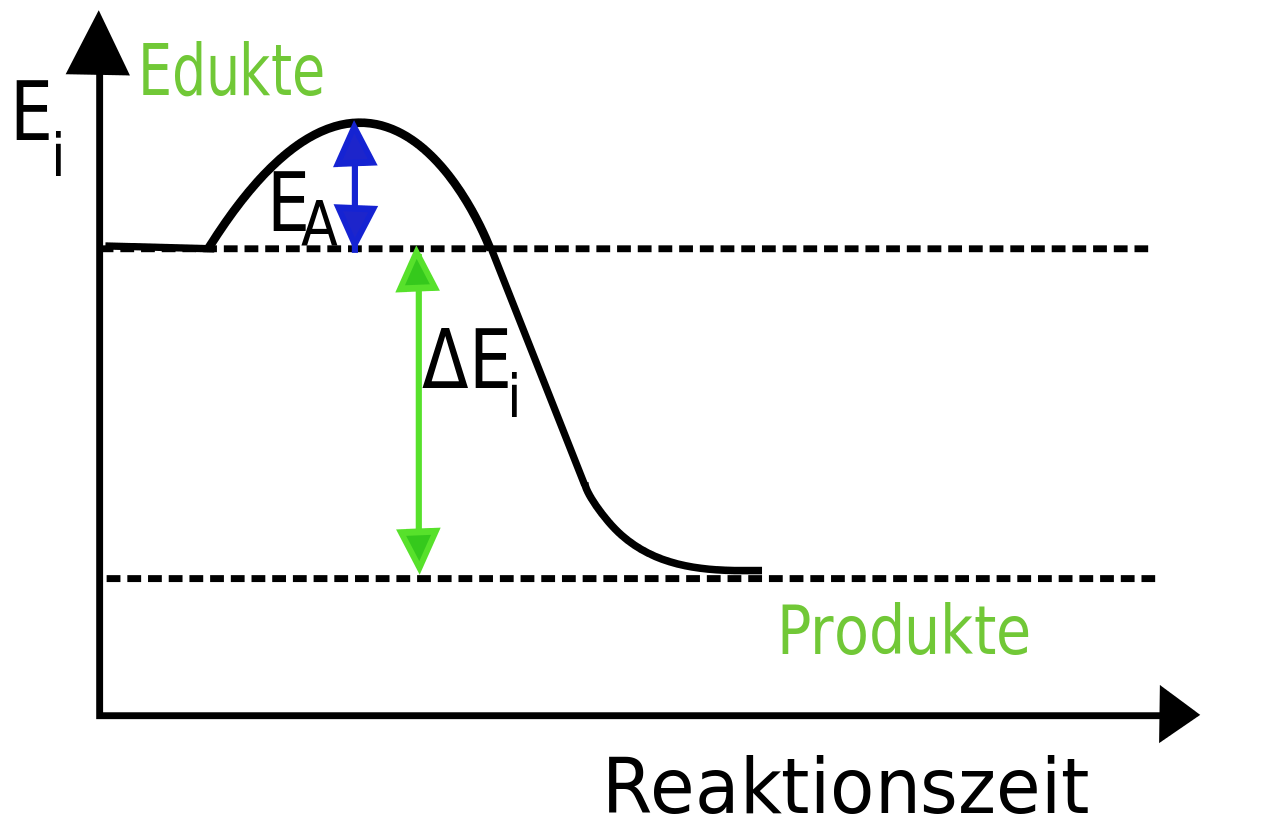
\includegraphics[width=0.6\columnwidth]{../exotherm_enthalpie.png}
	\end{figure}
	\begin{itemize}
		\item<+-> $\Delta E_i = \Delta H_R < 0 \implies$ Exotherm
		\item<+-> Energie wird freigesetzt
	\end{itemize}
	\end{block}
	\end{column}
	\begin{column}<+->{0.48\textwidth}
	\begin{block}{Endotherm}
	\begin{figure}[H]
		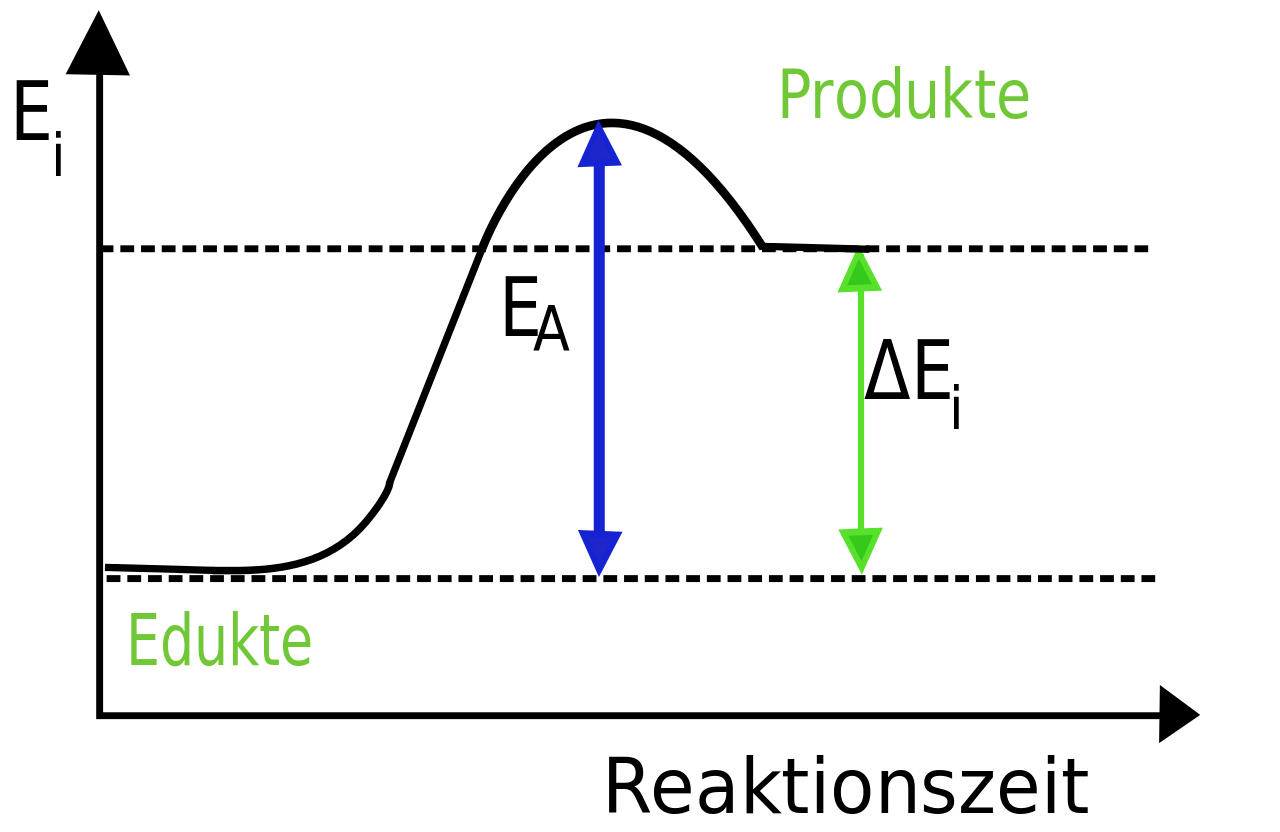
\includegraphics[width=0.6\columnwidth]{../endotherm_enthalpie.png}
	\end{figure}
	\begin{itemize}
		\item<+-> $\Delta E_i = \Delta H_R > 0 \implies$ Endotherm
		\item<+-> Energie wird aufgenommen
	\end{itemize}
	\end{block}
	\end{column}
	\end{columns}
	\begin{block}{Eigenschaften}
	\begin{itemize}
		\item<+-> $E_A$ bezeichnet die Aktivierungsenergie, die benötigt wird, um die Reaktion zu starten 
	\end{itemize}
	\end{block}

\section{radikalische Substitution}

\begin{itemize}
	\item<+-> Wasserstoffatome werden von Alkanen abgespalten
	\item<+-> werden ersetzt/substituiert durch Halogenatome (Fluor (\ch{F}), Chlor (\ch{Cl}), Brom (\ch{Br}), Iod (\ch{I}))
	\item<+-> Benötigt zum Kettenstart externe Energie, um Radikale zu erzeugen (Sonnenlicht, Hitze, etc.)
\end{itemize}


\begin{block}{Kettenstart / Initation}
\begin{itemize}
	\item<+-> Hydrolytische Aufbrechung vom Brom
	\item<+-> Zuführung von Energie (Licht, Wärme)
	\item<+-> Bindungspartner behalten Elektronen
\end{itemize}
\end{block}
\begin{examples}
	\schemestart
		\chemfig{\charge{180=\|,90=\|,-90=\|}{Br}-\charge{0=\|,90=\|,-90=\|}{Br}}
		\arrow{->[*{0}$E_{\text{Light}}$][]}[-90, 0.8]
		2 \chemfig{\charge{180=\|,90=\|,-90=\|,0=.}{Br}}
		\arrow{->[*{0}+ 2 \chemfig{C_6H_{13}-[0,0.6]C(-[2,0.6]H)(-[-2,0.6]H)-[0,0.6]H}][]}[-90, 1]
		2 \chemfig{C_6H_{13}-[0,0.6]\charge{0=.}{C}(-[2,0.6]H)(-[-2,0.6]H)} \+ 
		2 \chemfig{H-[0,0.6]\charge{[overlay=false]90=\|,0=\|,-90=\|}{Br}}
	\schemestop
\end{examples}

\begin{block}<+->{Kettenfortschritt / Folgereaktion / Prolongation}
\begin{itemize}
	\item Reaktion mit Kohlenwasserstoff
	\item<+-> Bildung weiterer Radikale, es entsteht \chemfig{H-\charge{[overlay=false]90=\|,0=\|,-90=\|}{Br}} und ein Alkylradikal
	\item<+-> Reaktion mit unreagierten Halogenmolekül, es entsteht ein Halogenalkan
	\item<+-> Wiederholen dieses Schrittes bis kein Edukt mehr vorliegt
\end{itemize}
\end{block}
\begin{examples}
	\schemestart
		\chemfig{@{start}\charge{180=\|,90=\|,-90=\|,0=.}{Br}}
		\arrow{->[*{0}+ \chemfig{C_6H_{13}-[0,0.6]C(-[2,0.6]H)(-[-2,0.6]H)-[0,0.6]H}][]}[-90, 0.8]
		\chemfig{C_6H_{13}-[0,0.6]\charge{0=.}{C}(-[2,0.6]H)(-[-2,0.6]H)} \+ 
		\chemfig{H-[0,0.6]\charge{[overlay=false]90=\|,0=\|,-90=\|}{Br}}
		\arrow{->[*{0}+ \chemfig{\charge{180=\|,90=\|,-90=\|}{Br}-[0,0.6]\charge{0=\|,90=\|,-90=\|}{Br}}][]}[-90, 0.6]
		\chemfig{C_6H_{13}-[0,0.6]C(-[2,0.6]H)(-[-2,0.6]H)-[0,0.6]\charge{0=\|,90=\|,-90=\|}{Br}} \+ 
		\chemfig{@{end}\charge{180=\|,90=\|,-90=\|,0=.}{Br}}
		\chemmove[-stealth,blue]{
			\draw ([yshift=3pt,xshift=3pt]end.45) .. controls +(350:20pt) and +(10:150pt) .. (start.45);
		}
	\schemestop
\end{examples}

\begin{block}{Kettenabbruch}
\begin{itemize}
	\item<8-> Rekombination der Radikale (Bildung von Konvalenten Bindungen):
	\item<9-> Zwei Halogenradikale treffen aufeinander
	\item<10-> Ein Halogenradikal und ein Alkylradikal treffen aufeinander
	\item<11-> Zwei Alkylradikale treffen aufeinander
	\item<12-> Notiz: Da die Rekombination energetisch ungünstig ist, spielt der Kettenabbruch bis die Edukte verbraucht sind meist eine untergeordnete Rolle.
\end{itemize}
\end{block}
\begin{examples}
	\schemestart
		2 $\cdot$ \chemfig{@{bro}\charge{180=\|,90=\|,-90=\|,0=.}{Br}}
		\chemmove[red,-stealth]{
			\draw ([xshift=4pt]bro.350) .. controls +(315:10pt) and +(45:10pt) .. ([xshift=4pt]bro.10);
		}
		\arrow(br--){->}
		\chemfig{\charge{180=\|,90=\|,-90=\|}{Br}-\charge{0=\|,90=\|,-90=\|}{Br}}
		\arrow(@br--kyl){0}[-90]
		\chemfig{C_6H_{13}-[0,0.6]@{c}\charge{0=.}{C}(-[2,0.6]H)(-[-2,0.6]H)}
		\arrow(@kyl--){->[+ \chemfig{@{br}\charge{0=\|,90=\|,-90=\|,180=.}{Br}}]}
		\chemmove[red, -stealth] {
			\draw ([xshift=-2pt]br.180) .. controls +(120:10pt) and +(60:10pt) .. ([xshift=2pt]c.10);
		}
		\chemfig{C_6H_{13}-[0,0.6]C(-[2,0.6]H)(-[-2,0.6]H)-[0,0.6]\charge{0=\|,90=\|,-90=\|}{Br}}
		\arrow(@kyl--kyl2){0}[-90]
		2 $\cdot$ \chemfig{C_6H_{13}-[0,0.6]@{cro}\charge{0=.}{C}(-[2,0.6]H)(-[-2,0.6]H)}
		\chemmove[red,-stealth]{
			\draw ([xshift=4pt]cro.350) .. controls +(315:10pt) and +(45:10pt) .. ([xshift=4pt]cro.10);
		}
		\arrow(@kyl2--){->}
		\chemfig{C_6H_{13}-[0,0.6]C(-[2,0.6]H)(-[-2,0.6]H)-[0,0.6]C(-[2,0.6]H)(-[-2,0.6]H)-[0,0.6]C_6H_{13}}
	\schemestop
\end{examples}


\section{elektrophile Addition}

	\begin{block}{Mechanismus}
	\begin{itemize}
		\item<+-> Ungesättigte Kohlenwasserstoffe wie Alkene oder Alkine reagieren mit Halogenen
		\item<+-> Halogene greifen Doppelbindung im Substrat an
		\item<+-> Unterteilung in mehrere Schritte (siehe folgendes Beispiel)
	\end{itemize}
	\end{block}
	\begin{alertblock}<+->{Halogene}
		Die elektrophile Addition funktioniert ausschließlich mit Chlor (\ch{Cl}), Brom (\ch{Br}) und Iod (\ch{I}), da Fluor (\ch{F}) so elektronegativ ist, dass es die \chemfig{C-C}-Bindung und die \chemfig{C-H}-Bindung im Alken/Alkin angreift.
	\end{alertblock}


\begin{examples}[+ \chemfig{X_2}]
\schemestart
	\chemfig{R^1-[1]C=[@{b1}]C-[-1]R^2}
	\arrow{->[\chemfig{@{ax}X_2}]}
	\chemmove[red,-stealth]{
		\draw (ax.90) .. controls +(120:30pt) and +(70:20pt) .. (b1.90);
	}
	\chemfig{R_1-[1]C(-[1.2,0.8506,,,draw=none]@{br1}X-[2]X)=[@{bond}]C-[-1]R^2}
	\chemmove[black, dashed, -]{
		\draw (bond.90) -- (br1);
	}
	\arrow{->[-\chemfig{X^\fminus}]}[-90]
	\chemfig{R_1-[1]C(<[1.2,0.8506]\charge{-90:10pt=\scrp}{X})=C(<[2.8,0.8506]\phantom{X})-[-1]R^2}
	\arrow{->[+ \chemfig{@{hadd}X^\fminus}]}[180]
	\chemfig{R_1-[1]C(<[3]X)-[@{bond}]C(<:[1]@{hadd2}X)-[-1]R^2}
	\chemmove[red,-stealth]{
		\draw (hadd.110) .. controls +(315:5pt) and +(120:5pt) .. (hadd2.340);
	}
\schemestop
\begin{itemize}
	\item Halogenmolekül wird polarisiert, das dem Alken/-in zugewandte Halogen-Atom wird partiell postiv und das abgewandte partiell negativ geladen
	\item Halogen-Kation addiert sich nun an die Doppelbindung des Alkens/-ins
	\item es entsteht ein negativ geladenes Halogen-Ion
	\item Das negativ-geladene Halogen-Ion greift nun an der anderen Seite des ehemaligen Ethen-Moleküls an
	\item Die \say{Doppelbindung} zum obrigen Halogen-Kation wird gelöst und verbindet sich mit dem Halogen-Ion.
\end{itemize}

\end{examples}



\begin{examples}[+ \chemfig{XH}]
\schemestart
	\chemfig{R^1-[1]C=[@{b1}]C-[-1]R^2}
	\arrow{->[\chemfig{@{ax}XH}]}
	\chemmove[red,-stealth]{
		\draw (ax.90) .. controls +(120:30pt) and +(70:20pt) .. (b1.90);
	}
	\chemfig{R_1-[1]C(-[1.2,0.8506,,,draw=none]@{br1}X-[2]H)=[@{bond}]C-[-1]R^2}
	\chemmove[black, dashed, -]{
		\draw (bond.90) -- (br1);
	}
	\arrow{->[-\chemfig{H^\fminus}]}[-90]
	\chemfig{R_1-[1]C(<[1.2,0.8506]\charge{-90:10pt=\scrp}{X})=C(<[2.8,0.8506]\phantom{X})-[-1]R^2}
	\arrow{->[+ \chemfig{@{hadd}H^\fminus}]}[180]
	\chemfig{R_1-[1]C(<[3]X)-[@{bond}]C(<:[1]@{hadd2}H)-[-1]R^2}
	\chemmove[red,-stealth]{
		\draw (hadd.110) .. controls +(315:5pt) and +(120:5pt) .. (hadd2.340);
	}
\schemestop
\end{examples}

\section{Eliminierung}

	\begin{itemize}
		\item \say{elektrophile Addition rückwärts}
		\item<+-> Spaltet \ch{X-H} ab
		\item<+-> 3 verschiedene Mechanismen: $E_1$, $E_1cB$, $E_2$
	\end{itemize}

\subsection*{$E_1$}
\begin{examples}
\schemestart
	\chemfig{C(-[3]H_3C)(<:[1.5]CH_3)(<[0.3]H)-[-2]C(-[-1]CH_3)(<:[@{xb}-2.8]@{xm}X)<[-3.8]H_3C}
	\chemmove[red,-stealth]{
		\draw ([xshift=2pt]xb.330) .. controls +(320:15pt) and +(355:10pt) .. (xm.315);
	}
	\arrow{->[][- \chemfig{X^\fminus}]}
	\chemfig{C(-[3]H_3C)(<:[1.5]CH_3)(<[@{hb}0.3]H)-[@{ccb}-2]\charge{-90:8pt=\fscrp}{C}(-[-1]CH_3)-[-3]H_3C}
	\chemmove[red,-stealth]{
		\draw (hb.270) .. controls +(270:10pt) and +(0:10pt) .. (ccb.0);
	}
	\arrow{->[][- \chemfig{H^\fplus}]}
	\chemfig{C(-[3]H_3C)(-[1]CH_3)=[-2]C(-[-1]CH_3)-[-3]H_3C}
\schemestop
\end{examples}
\begin{block}<+->{Vorgang}
\begin{itemize}
	\item Das Halogen-Atom wird im ersten Schritt abgespalten
	\item<+-> Das Wasserstoff-Atom wird im zweiten Schritt abgespalten
\end{itemize}
\end{block}


\subsection*{$E_1cB$}
\begin{examples}
\schemestart
	\chemfig{C(-[3]H_3C)(<:[1.5]CH_3)(<[@{hb}0.3]H)-[@{ccb}-2]C(-[-1]CH_3)(<:[-2.8]X)<[-3.8]H_3C}
	\chemmove[red,-stealth]{
		\draw (hb.270) .. controls +(270:10pt) and +(0:10pt) .. (ccb.0);
	}
	\arrow{->[+ \chemfig{\charge{90=\|}{B}}][- \chemfig{HB^\fplus}]}
	\chemfig{\charge{-45:6pt=\fscrm}{C}(-[3]H_3C)(-[1]CH_3)-[@{ccb}-2]C(-[-1]CH_3)(<:[@{xb}-2.8]@{xm}X)<[-3.8]H_3C}
	\chemmove[red,-stealth]{
		\draw ([xshift=2pt]xb.330) .. controls +(320:15pt) and +(355:10pt) .. (xm.315);
	}
	\arrow{->[][- \chemfig{X^\fminus}]}
	\chemfig{C(-[3]H_3C)(-[1]CH_3)=[-2]C(-[-1]CH_3)-[-3]H_3C}
\schemestop
\end{examples}
\begin{block}<+->{Vorgang}
\begin{itemize}
	\item Das \textbf{Wasserstoff-Atom} wird im \textbf{ersten} Schritt abgespalten
	\item<+-> Das \textbf{Halogen-Atom} wird im \textbf{zweiten} Schritt abgespalten
\end{itemize}
\end{block}


\subsection*{$E_2$}
\begin{examples}
\schemestart
	\chemfig{C(-[3]H_3C)(<:[1.5]CH_3)(<[@{hb}0.3]H)-[@{ccb}-2]C(-[-1]CH_3)(<:[@{xb}-2.8]@{xm}X)<[-3.8]H_3C}
	\chemmove[red,-stealth]{
		\draw (hb.270) .. controls +(270:10pt) and +(0:10pt) .. (ccb.0);
		\draw ([xshift=2pt]xb.330) .. controls +(320:15pt) and +(355:10pt) .. (xm.315);
	}
	\arrow{->[+ \chemfig{\charge{90=\|}{B}}][\subscheme{ - \chemfig{HB^\fplus} \arrow(--){0}[-90,0.1] - \chemfig{X^\fminus} }]}
	\chemfig{C(-[3]H_3C)(-[1]CH_3)=[-2]C(-[-1]CH_3)-[-3]H_3C}
\schemestop
\end{examples}
\begin{block}<+->{Vorgang}
\begin{itemize}
	\item Das Wasserstoff-Atom und das Halogen-Atom wird in \textbf{einem Schritt} abgespalten
\end{itemize}
\end{block}


\subsection*{Reaktionsgeschwindigkeit}
\begin{alertblock}{$E_1$ / $E_1cB$}
Da die $E_1$ / $E_1cB$-Reaktion in zwei Schritten verläuft, beeinflusst nur eine Konzentration die Reaktionsgeschwindigkeit (der 1. Schritt muss vollendet sein, damit der 2. Schritt passieren kann)
\begin{align*}
	v = k_1 \cdot c[\text{Substrat}]
\end{align*}
\end{alertblock}
\begin{alertblock}<+->{$E_1$ / $E_1cB$}
Da die $E_2$-Reaktion in einem Schritt verläuft, beeinflussen \textbf{beide} Konzentrationen die Reaktionsgeschwindigkeit (Beide Edukte sind am 1. Schritt beteiligt)
\begin{align*}
	v = k_2 \cdot c[\text{Substrat}] \cdot c[\text{Elektrophil}]
\end{align*}
\end{alertblock}

\section{nukleophile Substitution}

\subsection*{$S_N1$}
\begin{examples}
% \setchemfig{ scheme debug = true}
\schemestart
	\chemfig{
		X-[@{bond}-2](-[-3]R^1)(<:[-1]R^2)<[-1.7]R^3 
	}
	\chemmove[red,-stealth]{
		\draw (bond.0) .. controls +(10:20 pt) and +(-80:10pt) .. ([yshift=18pt, xshift=17pt]bond.180);
	}
	\arrow{->}
	\chemfig{X^\fminus} \+
	\chemleft[
	\chemfig{R_1-@{anchormid}(<:[1]R_2)(<[-1]R_3)-[2,0.33,,,draw=none]\fscrp}
	\chemright]
	\arrow(aa--){->[+ \chemfig{^\fminus @{anchor1}Nu}]}[20]
	\chemmove[red,-stealth]{
		\draw ([yshift=12pt, xshift=-3pt]anchor1.110).. controls +(120:10pt) and +(150:80pt) ..(anchormid.90);
	}
	\chemfig{
		Nu-[-2](-[-3]R^1)(<:[-1]R^2)<[-1.7]R^3 
	}
	\arrow(@aa--){->[+ \chemfig{_\fminus @{anchor2}Nu}]}[-20]
	\chemmove[red,-stealth]{
		\draw ([yshift=-12pt, xshift=-3pt]anchor2.250).. controls +(240:10pt) and +(210:80pt) ..(anchormid.270);
	}
	\chemfig{
		Nu-[2](-[3]R^1)(<:[1]R^2)<[1.7]R^3 
	}
\schemestop
\end{examples}


\begin{block}{Schritte}
Die $S_N1$-Reaktion verläuft 2-Schrittig
\end{block}
\begin{alertblock}{Reaktionsgeschwindigkeit}
Bei einer $S_N1$-Reaktion beeinflusst \textbf{nur eine} Konzentration die Reaktionsgeschwindigkeit (weil sie in 2 Schritten verläuft)
\begin{align*}
	v &= k_1 \cdot c\left[\text{Substrat}\right]
\end{align*}
\end{alertblock}


\subsection*{$S_N2$}
\begin{examples}
% \setchemfig{ scheme debug = true}
\schemestart
	\chemfig{
		X-@{midpoint_1}(-[1.2]R^1)(<:[-1.2]R^2)<[-0.5]R^3 
	}
	\arrow{->[+ \chemfig{^{\fminus}@{charge}Nu}]}
	\chemmove[red,-stealth]{
		\draw ([yshift=4pt, xshift=-13pt]charge.120) .. controls +(120:5 pt) and +(15:20pt) .. (midpoint_1.0);
	}
	\chemleft[
		\chemfig{@{x}X-[@{bond}:0,,,,dashed](-[:0,,,,dashed]Nu)(-[2]R^1)(<[-1]R^3)<:[-3]R^2}
	\chemright]
	\chemmove[-stealth,red]{
		\draw (bond.90).. controls +(100:20 pt) and +(80:10pt) .. (x.45) ;
	}
	\chemmove{\node[] at (-3pt,43pt) {\fscrm};}
	\arrow(m--x){->}
	\chemfig{X^\fminus} \+
	\arrow(@x--r){0}[,0]
	\chemfig{R^1-[-1.8](<[-2.2]R^3)(<:[-3.2]R^2)-Nu}
\schemestop
\end{examples}


\begin{block}{Schritte}
Die $S_N2$-Reaktion verläuft 1-Schrittig
\end{block}
\begin{alertblock}{Reaktionsgeschwindigkeit}
Bei einer $S_N2$-Reaktion beeinflussen \textbf{beide} Konzentrationen die Reaktionsgeschwindigkeit (weil sie in einem Schritt verläuft)
\begin{align*}
	v &= k_2 \cdot c\left[\text{Substrat}\right] \cdot c\left[\text{Nukleophil}\right]
\end{align*}
\end{alertblock}


\chapter{Stoffklassen}


\begin{itemize}
	\item<+-> Einteilung von Stoffen
	\item<+-> funktionelle Gruppe ist charakteristisch für Stoffklasse
	\item<+-> Atome in Molekülen bestimmen über chemische und physikalische Eigenschaften
\end{itemize}



\begin{table}[H]
\begin{tabular}{l|l}
Funktionelle Gruppe & Stoffklasse   \\ \hline\hline
Halogen  \chemfig{R-[,0.65]X}           & Halogenalkane \\ \hline
Amino-Gruppe    \chemfig{R-[,0.65]N(-[1,0.65]H)-[-1,0.65]H}    & Amine         \\ \hline
Hydroxy-Gruppe   \chemfig{R-[,0.65]\charge{[overlay=false]-90=\|,90=\|}{O}-[,0.65]H}   & Alkohle       \\ \hline
Ether-Gruppe     \chemfig{R^1-[,0.65]\charge{[overlay=false]-90=\|,90=\|}{O}-[,0.65]R^2}   & Ether         \\ \hline
Aldehyd-Gruppe    \chemfig{R-[,0.65]C(=[1,0.65]\charge{[overlay=false]90=\|,0=\|}{O})-[-1,0.65]H}  & Aldehyde      \\ \hline
Keto-Gruppe     \chemfig{C(-[3,0.65]R^1)(=[,0.65]\charge{[overlay=false]45=\|,315=\|}{0})-[-3,0.65]R^2}    & Ketone        \\ \hline
Carboxy-Gruppe  \chemfig{C(-[-3,0.65]R)(=[2,0.65]\charge{[overlay=false]45=\|,135=\|}{0})-[-1,0.65]\charge{[overlay=false]-45=\|,-135=\|}{O}-[1,0.65]H}    & Carbonsäure  
\end{tabular}
\end{table}



\begin{alertblock}{Mehrere Stoffklassen}
	Einige Moleküle können auch mehrere Stoffklassen haben, zum Beispiel:

	\vspace{20pt}

	\chemname{\chemfig{NH_2-C(-[2]COOH)(-[-2]R)-H}}{Aminsäure}
\end{alertblock}


\chapter{Teste dich!}

\schemestart
	\chemfig{\charge{90=\|,-90=\|,180=\|}{Cl}-C(-[2]H)(-[-2]H)-C(-[2]H)(-[-2]H)-\charge{90=\|,45=\|}{O}-[-1]H}
\schemestop
\hspace{5em}
\schemestart
	\chemfig{H-C(-[2]H)(-[-2]H)-C(-[2]H)(-[-2]H)-\charge{0=\|}{N}(-[-1]H)-[1]H}
\schemestop

\vspace{5em}

\schemestart
	\chemfig{H-C(-[2]H)(-[-2]H)-C(-[2]H)(-[-2]H)-F}
\schemestop
\hspace{5em}
\schemestart
	\chemfig{H-C(-[2]C(-[2]H)(-[4]H)-H)(-[-2]C(-[-2]H)(-[4]H)-H)=\charge{45=\|,-45=\|}{O}}
\schemestop

\section{induktive Effekte}
\begin{task}
	Zeichne die Induktiven Effekte in die obrigen Moleküle ein!
\end{task}

\section{Stoffklassen}
\begin{task}
	Markiere in obrigen Molekülen die funktionellen Gruppen und ordne sie begründet in eine oder mehrere Stoffklassen ein!
\end{task}

\section{nukleophile Substitution}
\begin{task}
	Die Gabriel-Synthese ist ein Verfahren zur selektiven Herstellung primärer Amine. Ein Schritt behilft sich dabei der nukleophilen Substitution.

	Seien folgende Moleküle gegeben:

	\vspace{2em}
	\chemname{
		\chemfig{**6(--(*5(-(=[::-60]\charge{-45=\|,-135=\|}{O})-\charge{45=\fminus}{N}(-[0,,,,draw=none]\charge{45=\fplus}{K})-(=[::-60]\charge{45=\|,135=\|}{O})--))----)}
	}{Kaliumphthalimid}
	\hspace{100pt}
	\chemname{
		\chemfig{H_3C-C(-[2]CH_3)(-[-2]CH_3)-\charge{90=\|,-90=\|,0=\|}{Br}}
	}{2-Brom-2,2-Methanylethan}
	\vspace{2em}

	Gebe alle Reaktionsprodukte sowie den zugehörigen Mechanismus, unter der Annahme das primär die $S_N1$ stattfindet, an! Von der Konzentration welchen Moleküls ist die Reaktion primör abhängend?
\end{task}

\section{elektrophile Addition}
\begin{task}
Gebe den Reaktionsmechanismus für die elektrophile Addition von \chemfig{Br_2} sowie \chemfig{H-\charge{90=\|,-90=\|,0=\|}{Br}} an Ethen (das folgende Molekül) an:

\vspace{2em}
\chemname{
	\chemfig{C(-[-3]H)(-[3]H)=C(-[1]H)-[-1]H}
}{Ethen}

\end{task}

\begin{task}
	Begründe: Würde auch die Addition an Ethin funktionieren? Die Addition an Ethan?
\end{task}

\section{radikalische Substitution}
\begin{task}
Die Wohl-Ziegler-Reaktion stellt eine radikalische Bromierung von Alkenen dar. Gebe alle möglichen Produkte der Wohl-Ziegler-Reaktion mit Cyclohexen (das folgende Molekül) an!

\vspace{2em}
\chemname{
	\chemfig{*6(----=-)}
}{Cyclohexen}
\end{task}
\section{Eliminierung}
\begin{task}
2-Methylpropan-2-ol wird in einer sauren wässrigen Lösung gelöst. Zeichne die Moleküle und gebe den Reaktionsmechanismus der Eliminierung 1. Ordnung an.

Begründe, von welchen Molekülen die Reaktionsgeschwindigkeit abhängt.
\end{task}
\begin{task}
In einer Lösung liegen Brommethan und Hydroxid-Ionen vor. Zeichne die Moleküle und gebe den Reaktionsmechanismus der Eliminierung 2. Ordnung an.

Begründe, von welchen Molekülen die Reaktionsgeschwindigkeit abhängt.
\end{task}
